\documentclass{article}
\usepackage[utf8]{inputenc}
\usepackage[margin=1in,left=1.5in,includefoot]{geometry}
\usepackage{booktabs}
\usepackage{graphicx}
\usepackage{hyperref}

% Header & Footer Stuff

\usepackage{fancyhdr}
\pagestyle{fancy}
\lhead{Visión por Computador Aplicada}
\rhead{614G030332425}
% \fancyfoot{}
% \lfoot{Pablo Chantada Saborido \& José Romero Conde}
% \fancyfoot[R]{}

% The Main Document
\begin{document}
	\begin{center}
		\LARGE\bfseries PRÁCTICA II\\
		\small Pablo Chantada Saborido \& José Romero Conde
		\line(1,0){430}
	\end{center}
	
	
\section*{Modelo Baseline}

Describimos ahora nuestro modelo baseline, que nos valió para iterar y comparar resultados. El modelo se compone de los siguientes elementos:

\begin{itemize}
	\item Aumento de datos compuesto. (expñicar bien en algun suitio)
	\item  \href{https://arxiv.org/pdf/1905.11946}{Efficienet}. La usamos como CNN de partida.
	\item Un MLP de tres capas, sobre la salida de la red.
\end{itemize}

blñablabla como se ve en la figurta



\begin{figure}[h]
	\centering
	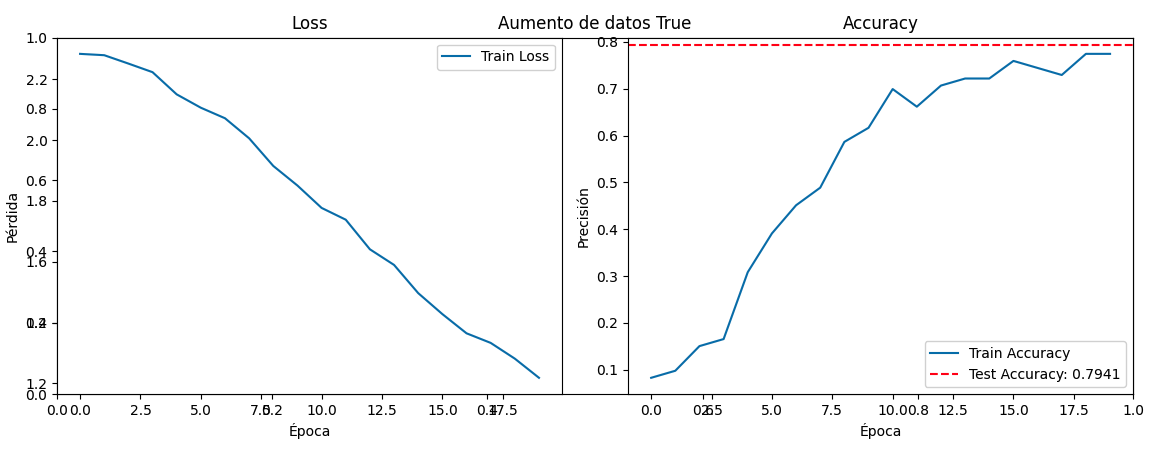
\includegraphics[width=0.7\linewidth]{baselineCon}
	\caption{}
	\label{fig:baselinecon}
\end{figure}

\begin{figure}[h]
	\centering
	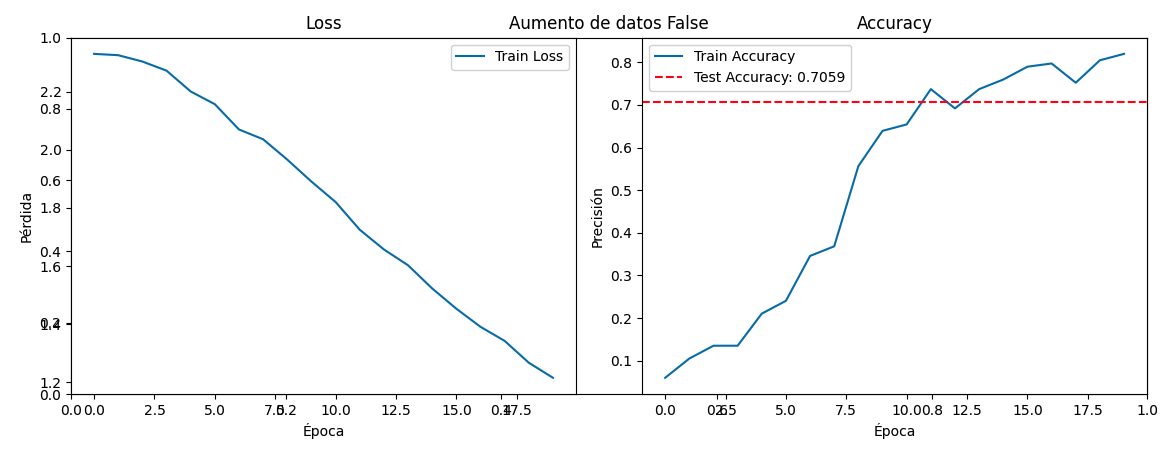
\includegraphics[width=0.7\linewidth]{baselineSin}
	\caption{}
	\label{fig:baselinesin}
\end{figure}


\section*{Cambios para el segundo ejercicio}

blablabla

\section*{ANEXO}
	\begin{figure}[h]
	\centering
	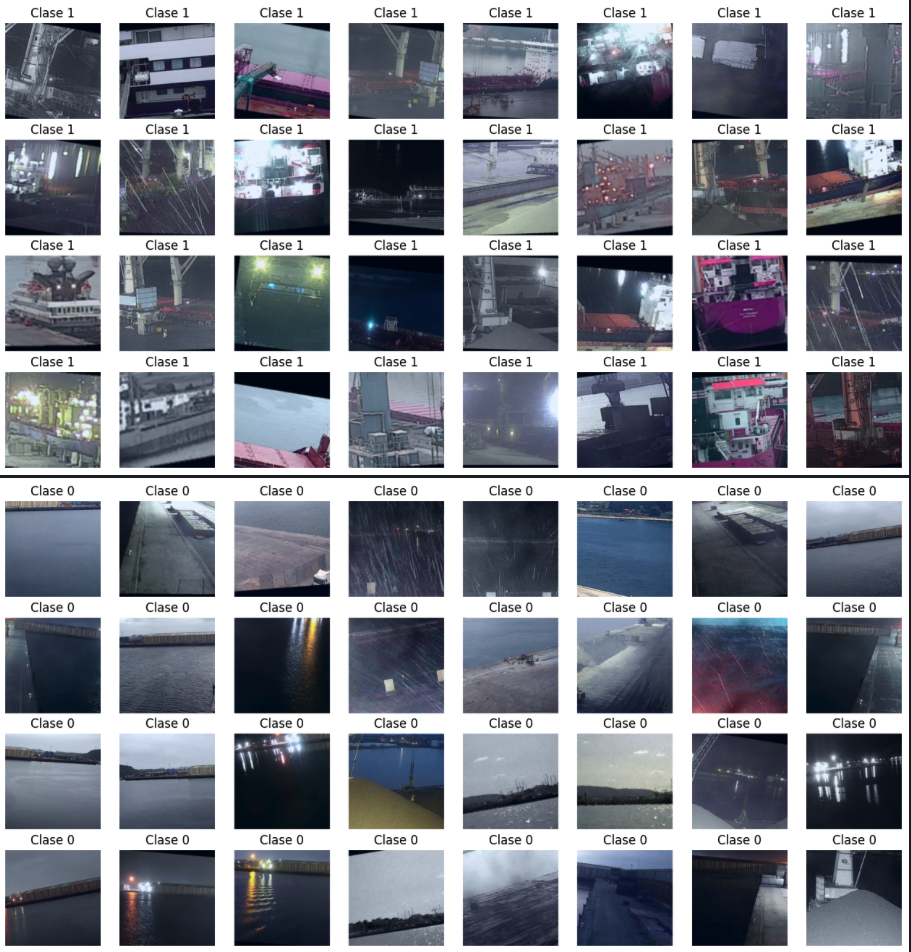
\includegraphics[width=0.6\linewidth]{imagenesCon}
	\caption{Imagenes con aumento de datos}
	\label{fig:imagenescon}
\end{figure}

\begin{figure}[h]
	\centering
	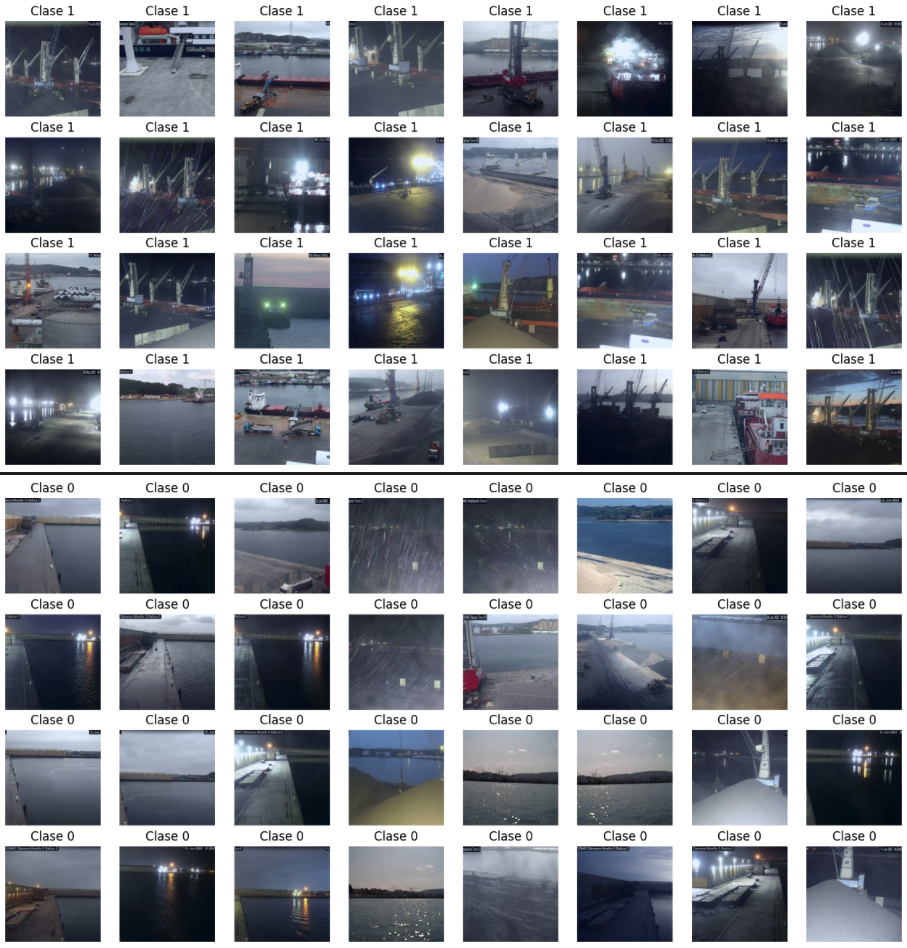
\includegraphics[width=0.6\linewidth]{imagenesSin}
	\caption{Imagenes sin aumento de datos}
	\label{fig:imagenessin}
\end{figure}

























\end{document}

